\documentclass[paper=a4,german,11pt,titlepage,twoside=false,headings=normal,numbers=noenddot,captions=tableabove,listof=totoc,index=totoc,bibliography=totoc,plainheadsepline,plainfootsepline]{scrreprt}
%-----------------------------------------------------------------
\usepackage{etoolbox}
\newbool{deutsch}
\booltrue{deutsch}
\hbadness=10000					% unterdrueckt unwichtige Fehlermeldungen
\vbadness=10000
%\pdfsuppresswarningpagegroup=1	% suppress stupid warnings originating from \includesvg
%-----------------------------------------------------------------
%\usepackage{amsmath} % abgesetzte Formeln zentriert in der Zeile
%\usepackage[fleqn,intlimits]{amsmath} % [fleqn] abgesetzte Formeln mit festem Abstand zum linken Rand
\usepackage[reqno,intlimits]{amsmath} % [reqno] um die gleichungsnummerierung rechts zu haben
% intlimits: Grenzen für Integrale unterhalb und oberhalb des Zeichens
\usepackage{amssymb}
\usepackage{array}
%\usepackage[ngerman]{babel}
%\usepackage[ngerman]{varioref}
\ifbool{deutsch}{%
    \usepackage[ngerman]{babel}
    \usepackage[ngerman]{varioref}
}{%
    \usepackage[english]{babel}
    \usepackage[english]{varioref}
}
\usepackage[T1]{fontenc} 
\usepackage[utf8]{inputenc}
%---------------------------
\usepackage{booktabs}
\usepackage{calc}
\usepackage{cancel}
\usepackage[labelfont={footnotesize,sf,bf},textfont={footnotesize,sf}]{caption} %Format (Textgröße, Textform) für Bildtext 
%normalsize
%scriptsize
% sc --> smallcaps
% bf --> bold face
% sf --> sans serif
%\usepackage{cite} %inkompatibel mit biblatex
\usepackage[table]{xcolor}
%\usepackage{colortbl}
\usepackage[right]{eurosym}
%\usepackage{caption2} %nicht zusammen mit sidecap
%\usepackage{exscale}
\usepackage{ellipsis}
\usepackage{graphicx}
\usepackage{float}
%\usepackage{floatflt}
%----------------------------------------
\usepackage{gensymb} %-----------
%\usepackage{helvet}
\usepackage{csquotes}
\usepackage{listings}
\usepackage{longtable}
\usepackage{lastpage}  %----------
\usepackage{lscape}
\usepackage{lmodern}  %-- Silbentrennung
%\usepackage{mathpazo} % andere mathematische Symbol
\usepackage{makeidx}
%\usepackage{minitoc}
\usepackage{multirow}
\usepackage{multicol}
%\usepackage[intoc]{nomencl}   % zwei Spalten beim Formelzeichenverzeichnis
\ifbool{deutsch}{%
    \usepackage[german,intoc]{nomentbl} %vier Spalten bei Formelzeichenverzeichnis
}{%
    \usepackage[english,intoc]{nomentbl} %vier Spalten bei Formelzeichenverzeichnis
}
\usepackage{nicefrac} %----
%\usepackage{picins} %----------
\usepackage{paralist} %--------
\usepackage{parallel}  %----------
\usepackage{pdfpages} %-------
% Define user colors using the RGB model
%\usepackage{colortbl}
%\definecolor{dunkelgrau}{rgb}{0.8,0.8,0.8}
%\definecolor{hellgrau}{rgb}{0.95,0.95,0.95}
%\usepackage{pgfplots}
\usepackage[figuresright]{rotating} 
\usepackage{scrlayer-scrpage}
%\usepackage[innercaption]{sidecap} %Beschriftung neben Bild, Tabelle, Mittelbach S333 %----------
%\usepackage{sistyle}
%\usepackage[locale=DE]{siunitx} %nicht zusammen mit sistyle %---------
\usepackage[locale=DE,per-mode=symbol,parse-numbers=false]{siunitx} %nicht zusammen mit sistyle %---------
% \usepackage[font={scriptsize,sl},captionskip=3pt]{subfig} % für die Unterbilder %---------
\usepackage{subcaption}
\usepackage{shortvrb}
\usepackage{tablefootnote}
\usepackage{tabularx}
\usepackage{tabulary}
\usepackage{textcomp}
\usepackage{tocbasic}
\usepackage{tikz}
\usepackage{times} 
\usepackage{units} %----------
\usepackage{xurl}
\usepackage{wrapfig} %----------
\usepackage{xr-hyper}
\usepackage{arydshln} %für \hdashline[5pt/2pt] % muss am Ende stehen, sonst gibt es Probleme mit xcolor
\usepackage[hidelinks]{hyperref} % muss am Schluss stehen
\hypersetup{linkcolor={0 1 1}, linkbordercolor={1 1 1}, citebordercolor={1 1 1}} % setzt Linkboxen auf Farbe "`weiß"'
%\usepackage{unicode-math}
%\usepackage[toc,symbols]{glossaries} %---------- muss nach hyperref stehen
\usepackage[nonumberlist, acronym, toc, section]{glossaries} % muss nach hypersetup stehen
%----------------
%\usepackage{romannum} % Seitenzahlen in römischen Ziffern
%\usepackage{adjustbox}
\usepackage{scrhack}
\usepackage[style=numeric, citestyle=numeric, backend=biber]{biblatex}
\usepackage[useregional]{datetime2}
\usepackage{cleveref} % löscht labels!!!!!!!!!! <--- warum? habs trotzdem eingefügt weil es die referencen nice macht ohne newcommands dafür zu brauchen. außerdem steht intellisense drauf ;)
\usepackage{isotope} % um chemische gleichungen hübscher darstellen zu können
\usepackage{framed} % rahmen um dinge malen können
\usepackage{svg} % um auch vektorgrafiken als bild einfügen zu können
\usepackage{adjustbox} % skaliert floats dynamischer (anti-over/underfull)
\usepackage[numbered]{bookmark} % platziert im pdf reader bei der kapitelübersicht die jeweiligen kapitelnummer vor die kapitelüberschriften
\usepackage{threeparttablex}
%===================== define VARIABLES ==========================
% --------------------- Names ------------------------------------
\newcommand{\thefirstnameA}{Cihan}
\newcommand{\thelastnameA}{Ünlü}
\newcommand{\thefirstnameB}{Dennis}
\newcommand{\thelastnameB}{Hunter}
\newcommand{\thefirstnameC}{Crack}
\newcommand{\thelastnameC}{Dough}
% --------------------- Titel Course -----------------------------
\newcommand{\titleLV}{Physikalische Chemie}
%---------------------- Document Titel ---------------------------
\newcommand{\subtitleA}{Praktikumsübung}
\newcommand{\subtitleB}{Nr. 10 und 11}
%---------------------- Dates ------------------------------------
% \newcommand{\versuch}{2} % Versuchsnummer einfügen
\newcommand{\dateLV}{31. Mai 2021} % Datum einfügen
\newcommand{\deadline}{14.6.2021} % Abgabedatum ist der 1.12.2020
% \newcommand{\dateLVa}{December 1st, 2020}
% \newcommand{\dateLVb}{December 8th, 2020}
%:::::::::::::::::::::::::::::::::::::::::::::::::::::::::::::::::
%-------------------------
 %\renewcommand{\captionlabelfont}{\sffamily} %für "Abbildung" und "Tabelle"
 %\renewcommand{\captionfont}{\sffamily\small} %für den Text der Bildunterschriften
%  \renewcommand{\captionlabelfont}{\sffamily} 
%  \renewcommand{\captionfont}{\sffamily} %\renewcommand{\normalfont}{\sffamily} %für die Überschriften
% Fettdruck der Bezeichnung Abbildung, Tabelle
%\renewcommand{\captionlabelfont}{\bfseries}
%---------------------------------------------
%------------------ Schrifttyp in der Kopf- und Fusszeilen
\setkomafont{pageheadfoot}{\footnotesize\sffamily}
%---------------------------------------------------
%Ändern der Abbildung- und Tabellenbezeichnung (Niedermair S.157)
%_____________________________________________
\ifbool{deutsch}{%
\addto\captionsngerman{\renewcommand\figurename{Abb.}}
\addto\captionsngerman{\renewcommand\tablename{Tab.}}
\renewcommand\listfigurename{Abbildungen}
}{}
%_______________________________
%Betrag eines Wertes
% \newcommand{\abs}[1]{\lvert #1 \rvert}
%---------------------------------------------
% \newcommand{\absatz}[1]{\textbf{\textsc{#1}}} %siehe Mittelbach S. 876ff
%----------------------------
%\newcommand{\absatz}{\par \medskip}
%______________________________
%\newcommand{\anhang}[1]{Anhang \ref{#1}, Seite \pageref{#1}}
% \newcommand{\anhang}[1]{Anhang \vref{#1}}
% %________________________________
% \newcommand{\aufgabe}{\stepcounter{plus} Aufgabe \arabic{plus}}
%______________________________________
%compactitem
% \newcommand{\bci}{\begin{compactitem}}
% \newcommand{\eci}{\end{compactitem}}
% %______________________________________
% %
% \newcommand{\bi}{\begin{itemize}}
% \newcommand{\ei}{\end{itemize}}
% %______________________________________
% %compactenumerate
% \newcommand{\bce}{\begin{compactenum}}
% \newcommand{\ece}{\end{compactenum}}
% %_____________________________________
% %begin equation
% \newcommand{\be}{\begin{equation}}
% \newcommand{\ee}{\end{equation}}
% %_____________________________________
% %begin equation ohne Formelnummer
% \newcommand{\ben}{\begin{equation*}}
% \newcommand{\een}{\end{equation*}}
% %_____________________________________
% %begin align ohne Formelnummer
% \newcommand{\ban}{\begin{align*}}
% \newcommand{\ean}{\end{align*}}
%_____________________________________
%begin align
% \newcommand{\ba}{\begin{align}}
% \newcommand{\ea}{\end{align}}
%_____________________________________
%minpage
% \newcommand{\bmp}{\begin{minipage}[t]{.47\linewidth}}
% \newcommand{\emp}{\end{minipage}}
%_____________________________
%  dB
% \newcommand{\db}{dB}
% %  dB(A)
% \newcommand{\dba}{ dB(A) }
% %  dB(A) für Satzende
% \newcommand{\dbap}{ dB(A)}
% %_________________________________
% \newcommand{\bzw}{bzw.\,}
% %_______________________________
% \newcommand{\dif}{\mathrm{d}}
%________________________________
% neuer Zähler
\newcounter{plus}
\setcounter{plus}{0}
%______________________________
%Für das Formelverzeichnis _____________________ Formelverzeichis ____
% Befehl umbenennen in fz
% \let\fz\nomenclature
% Deutsche Überschrift
\ifbool{deutsch}{%
\renewcommand{\nomname}{Formelzeichen}
}{}
% Punkte zw. Abkürzung und Erklärung
\setlength{\nomlabelwidth}{.20\hsize}
\renewcommand{\nomlabel}[1]{#1 \dotfill}
% Zeilenabstände verkleinern
\setlength{\nomitemsep}{-\parsep}
%_____________________________
% \newcommand{\bild}[1]{Abb. \vref{#1}}
% \newcommand{\sbild}[1]{siehe Abb. \vref{#1}}
% \newcommand{\bilder}[2]{Abb. \vrefrange{#1}{#2}}
% \newcommand{\bildseite}[1]{Abb. \vref{#1}} % erzeugt "`Abb. nn auf Seite nn
% \newcommand{\tabelle}[1]{Tab. \vref{#1}}
% \newcommand{\tabellenseite}[1]{Tab. \vref{#1}} % erzeugt "`Tab. nn auf Seite nn
% für \vref ist usepackage[german]{varioref} einzufügen
%_-------------------------------- Freiraum
% \newcommand{\freiraum}[1]{\begin{figure}[H]\vspace{#1\textheight}\end{figure}}
%_____________________________
% Gleichung
% \newcommand{\gl}[1]{Gl.\,(\ref{#1})}
% \newcommand{\sgl}[1]{siehe Gl.\,(\ref{#1})}
% \newcommand{\glbereich}[2]{Gl. \vrefrange[]{#1}{#2}}
%_____________________________
% Grad Celsius
% \newcommand{\grad}{\,\degC}
% \newcommand{\gradC}{\,\degree}
%______________________________________
% Großbuchstaben als Indizes kleiner schreiben; spezielle im Mathemodus
% \newcommand{\klein}[1]{\scriptscriptstyle{#1}}% Fettdruck der Bezeichnung 
%______________________________
%% Kasten
% \newcommand{\kasten}{\fbox{\rule{0.0pt}{10pt}{{ } } }}
%______________________________
%\newcommand{\kapitel}[1]{Kapitel \ref{#1}, Seite \pageref{#1}}
% \newcommand{\kapitel}[1]{Kapitel \vref{#1}}
%_____________________________
%  LAeq für den äquivalenten Dauerschallpegel
% \newcommand{\laeq}{ $L_{Aeq}$ }
%  LAeq für den äquivalenten Dauerschallpegel am Satzende
% \newcommand{\laeqp}{ $L_{Aeq}$}
%_________________________________
%   Linie zeichnen
\newcommand{\linie}{\rule{0.5\textwidth}{0.1pt}}
%---------------------- LaTeX
% \newcommand{\lt}{\LaTeX\,\,}
%----------------------------
% \newcommand{\nl}{\newline}
%__________________________________
%  multicolumn für Tabellen
% \newcommand{\mc}{\multicolumn}
%% \mc{1}{c}{Text}
%_________________________________
%    Parallel
% \newcommand{\pl}[1]{\ParallelLText{#1}}
% \newcommand{\pr}[1]{\ParallelRText{#1}}
% \newcommand{\pp}{\ParallelPar}
%------------ rot unterstrichen
% \newcommand{\rotunterstrichen}[1]{\textcolor{red}{\underline{\textcolor{black}{#1}}}}
%________________ Realteil
% \newcommand{\real}[1]{\text{Re}\left\{#1\right\}}
%________________________________--
% \newcommand{\seite}[1]{Seite \pageref{#1}}
% \newcommand{\seiten}[2]{\vpagerefrange{#1}{#2}}
%----------------------------
%        TEXT Rot
\newcommand{\textrot}[1]{\textcolor{red}{#1}}
%______________________________
%Abkürzung für \multicolumn
% \newcommand{\tab}[2]{\multicolumn{1}{#1}{#2}}
%_____________________________________
% doppelt unterstreichen
% \newcommand{\unterstreichen}[1]{\underline{\underline{#1}}}
% einfach unterstreichen
% \newcommand{\ul}[1]{\underline{#1}}
%______________________________
%kurze Verbatimausgabe
%\MakeShortVerb{\|} %mittelbach S.160 mit \usepackage{shortvrb}
%_______________________________________
% vspace
% \newcommand{\vsf}{\vspace{5pt}}
%_________________________________
% \newcommand{\zb}{z.B.\,}
% \newcommand{\idr}{i.d.R.\,}
%_______________________________
% Zähler-einfach
\newcounter{req}
% \newcommand{\zaehler}[1]{\refstepcounter{req}{#1} \thereq}
%% Beispielaufzählung \zaehler{Beispiel}\\
%_____________________________________
 \setlength{\voffset}{-2.532 cm}
 \setlength{\hoffset}{-1.57 cm}
% \setlength{\topmargin}{2.0 cm} \setlength{\topskip}{0.1 cm}
 \setlength{\topmargin}{1.5 cm}
 \setlength{\topskip}{0.1 cm}
 \setlength{\evensidemargin}{1.5 cm}
 \setlength{\oddsidemargin}{1.5 cm}
 \setlength{\textwidth}{16.5 cm}
 \setlength{\footskip}{40pt}
 \setlength{\textheight}{24.5cm}
% \setlength{\textheight}{23.5 cm}
 \setcounter{page}{1}
 \setlength{\parindent}{0cm}
 \setlength{\headsep}{20pt}
%----------------------------------------------------------------------
% Linien in der Kopf- und Fußzeile
%\renewcommand{\headrulewidth}{0.0pt}   %Linie in der Kopfzeile mit 0.0pt keine Linie
%%\renewcommand{\footrulewidth}{0.0pt}   %Linie in der Fußzeile mit 0.0 pt keine Linie
%\renewcommand{\headrulewidth}{0.2pt}   %Linie in der Kopfzeile mit 0.0pt keine Linie
%\renewcommand{\footrulewidth}{0.2pt}   %Linie in der Fußzeile mit 0.0 pt keine Linie
%------------------------------------------------------------------------
%\renewcommand{\normalfont}{\sffamily} %für die Überschriften
%\renewcommand{\chaptermark}[1]{\markboth{\chaptername\ \thechapter #1}{}}
%\renewcommand{\sectionmark}[1]{\markright{\thesection\ #1}}
% \rfoot{\leftmark\\\rightmark}

%Definitionen für Kopfzeile
% bei documentclass {report} hat der Eintrag für die [gerade Seite] keine Wirkung
%-------------------------------------------------------------
%%
%Einstellungen für Kopf- und Fusszeilen mit dem KOMA-Skript und \usepackage{scrpage2}
\pagestyle{scrheadings}
%\pagestyle{scrplain}
% le --> links, gerade Seite
% ce --> mittig, gerade Seite
% re --> rechts, gerade Seite
% lo --> links, ungerade Seite
% co --> mittig, ungerade Seite
% ro --> rechts, ungerade Seite
%---------------------------------------------
% Löschen aller Einträge
%\clearscrheadings
% \automark[section]{subsection}
% \pagemark --> Seitenzahl
% \automark --> Kapitelüberschriften
% \leftmark --> ??
% \rightmark --> ??
%::::::::::::::::::::::::::::::::::: Kopfzeile
% Kopfzeile gerade Seite
\automark[chapter]{chapter}
\lehead[]{\titelkopfzeilelinkseven}
\cehead[]{\titelkopfzeilemitteeven}
\rehead[]{\titelkopfzeilerechtseven}
% Kopfzeile ungerade Seite
\lohead[]{\titelkopfzeilelinksodd}
\cohead[]{\titelkopfzeilemitteodd}
\rohead[]{\titelkopfzeilerechtsodd}
% Linie in der Kopfzeile
%\setheadtopline{0.2pt} % obere Linie in der Kopfzeile; nur bei scrartcl
%\setheadsepline{0.4pt} % untere Linie in der Kopfzeile; nur bei scrartcl
\KOMAoptions{headsepline=0.4pt}
% Linie in der Fusszeile
%::::::::::::::::::::::::::::::::::: Fußzeile
% Fusszeile gerade Seite[plain-style]{scrheadings-style}
\lefoot[]{\titelfusszeilelinkseven} 
\cefoot[]{\titelfusszeilemitteeven}
\refoot[]{\titelfusszeilerechtseven}
% Fusszeile ungerade Seite
\lofoot[]{\titelfusszeilelinksodd}
\cofoot[]{\titelfusszeilemitteodd}
\rofoot[]{\titelfusszeilerechtsodd}
%\rofoot[\thepage ]{\thepage}
%\setfoottopline{0.2pt} % obere Linie in der Kopfzeile; nur bei scrartcl
%\setfootsepline{0.4pt} % untere Linie in der Kopfzeile; nur bei scrartcl
\KOMAoptions{footsepline=0.4pt}

% le --> links, gerade Seite
% ce --> mittig, gerade Seite
% re --> rechts, gerade Seite
% lo --> links, ungerade Seite
% co --> mittig, ungerade Seite
% ro --> rechts, ungerade Seite
% even --> gerade Seite
% odd --> ungerade Seite
%----------------------------------------- Kopfzeilentext
\newcommand{\titelkopfzeilemitteeven}{}
\newcommand{\titelkopfzeilemitteodd}{}
\newcommand{\titelkopfzeilelinkseven}{Hochschule RheinMain}
\newcommand{\titelkopfzeilelinksodd}{Hochschule RheinMain}
\newcommand{\titelkopfzeilerechtseven}{}
\newcommand{\titelkopfzeilerechtsodd}{}
%----------------------------------------- Fußzeilentext
\newcommand{\titelfusszeilemitteeven}{}
\newcommand{\titelfusszeilemitteodd}{}
\newcommand{\titelfusszeilerechtseven}{Studienbereich Angewandte Physik \& Medizintechnik}
\newcommand{\titelfusszeilerechtsodd}{Studienbereich Angewandte Physik \& Medizintechnik}
\newcommand{\titelfusszeilelinkseven}{\thepage \hspace{0.5mm} von \pageref{LastPage}}
\newcommand{\titelfusszeilelinksodd}{\thepage \hspace{0.5mm} von \pageref{LastPage}}
%
%=====================Code Listing Layout Matlab=============================
\definecolor{codegreen}{RGB}{28,172,0} % color values Red, Green, Blue
\definecolor{codelilas}{RGB}{170,55,241}
\lstdefinestyle{matlab}{language=Matlab,%
    basicstyle=\footnotesize,%
    inputencoding=latin1,%
    breaklines=true,%
    stepnumber=2,% line numbering steps
    morekeywords={ones,height,width,datetime},% additional keywords to highlight
    keywordstyle=\color{blue},%
    frame=none,%
    identifierstyle=\color{black},%
    stringstyle=\color{codelilas},%
    commentstyle=\color{codegreen},%
    showstringspaces=false,%without this there will be a symbol in the places where there is a space
    numbers=left,%
    numberstyle={\tiny \color{black}},% size of the numbers
    numbersep=9pt,% this defines how far the numbers are from the text
}
\lstdefinestyle{python}{language=Python,%
    basicstyle=\footnotesize,%
    inputencoding=latin1,%
    breaklines=true,%
    stepnumber=2,% line numbering steps
    morekeywords={ones,height,width,datetime},% additional keywords to highlight
    keywordstyle=\color{blue},%
    frame=none,%
    identifierstyle=\color{black},%
    stringstyle=\color{codelilas},%
    commentstyle=\color{codegreen},%
    showstringspaces=false,%without this there will be a symbol in the places where there is a space
    numbers=left,%
    numberstyle={\tiny \color{black}},% size of the numbers
    numbersep=9pt,% this defines how far the numbers are from the text
}
%==============================================================================
\DeclareNameAlias{author}{family-given}
\DeclareNameAlias{editor}{family-given}
\DeclareNameAlias{translator}{family-given}
\addbibresource{quellen.bib}
\chemsetup{
	modules = {reactions},
	formula = chemformula,
	reactions/tag-open=(R,
	reactions/tag-close=),
}
% \usepackage{showframe}
\usepackage[]{geometry}
\begin{document}
%-----------------------------------------------------------------
\newgeometry{text={17cm,22.5cm},left=2cm,right=2cm,bottom=2.5cm, headsep=1cm,includeheadfoot}
\begin{titlepage}
	% -------- Naming ------------------------------
	\ifbool{deutsch}{%
		\newcommand{\nameA}{\thefirstnameA\space\thelastnameA}
		\newcommand{\nameB}{\thefirstnameB\space\thelastnameB}
		\newcommand{\nameC}{\thefirstnameC\space\thelastnameC}
	}{%
		\newcommand{\nameA}{\thelastnameA\,\space\thefirstnameA}
		\newcommand{\nameB}{\thelastnameB\,\space\thefirstnameB}
		\newcommand{\nameC}{\thelastnameC\,\space\thefirstnameC}
	}
	% ----------------------------------------------
	\newcommand{\HRule}{\rule{\linewidth}{0.5mm}}
	\centering
	\textsc{\Large Hochschule RheinMain} \par
	\begin{center}
		
\includegraphics[width=0.15\textwidth]{logo-hsrm.jpg}
	\end{center}
	\textsc{\LARGE \titleLV}\vspace{0.5cm}
		\HRule\vspace{0.4cm}
	{\huge\bfseries \subtitleA}\par\vspace{0.4cm} % Title of Document
	{\huge\bfseries \subtitleB}\par\vspace{0.4cm} % Titel des Dokuments
		\HRule\vspace{1.5cm}
%-------------------
\begin{minipage}{0.4\textwidth}
	\large
	\ifbool{deutsch}{%
		\textit{\underline{Autoren}}\par\vspace{0.5cm}
	}{%
		\textit{\underline{Author}}\par\vspace{0.5cm}
	}
	\textsc{\nameA}\par\vspace{0.5cm}
	\textsc{\nameB}\par\vspace{0.5cm}
	% \textsc{\nameC}\par\vspace{0.5cm}
\end{minipage}
%------------------------------------
\vfill\vfill\vfill
\ifbool{deutsch}{%
	\textsc{\Large Fachbereich Ingenieurwissenschaften}\vspace{0.5cm}\par
	\textsc{\large Studienbereich Angewandte Physik \& Medizintechnik}\vspace{0.5cm}
	\vfill
	\begin{flushleft}
		Datum LV:\hspace{0.4cm} {\large\dateLV}\hspace{1cm}Datum der Abgabe:\hspace{0.4cm} {\large\today}
	\end{flushleft}
}{%
	\textsc{\Large Department of Engineering}\par\vspace{0.5cm}\par
	\textsc{\large Applied Physics \& Medical Technology}\par\vspace{0.5cm}
	\vfill
	\begin{flushleft}
		Date:\hspace{0.4cm} {\large\today}
	\end{flushleft}
}
\end{titlepage}
\tableofcontents
\clearpage
\pagenumbering{arabic}
%-----------------------------------------------------------------
% \newcommand{\chaptercount}{5} % put number of chapters here
% \foreach \c in {1,...,\chaptercount}{\input{chapters/\c_chap}}
\newgeometry{text={15cm,22.5cm},left=2cm,right=4cm, headsep=1cm}
%LTeX: language=de-DE
\chapter{Vorwort}
	Nachfolgend handelt es sich um zwei komplementäre Versuche -- namentlich Versuch 10 \textit{Konduktometrische Fällungstitration}
	und Versuch 11 \textit{Kalorimeteraufschluss}. Dementsprechend werden an dieser Stelle die Laborberichte in kombinierter Form
	bearbeitet.
%ltex: language=de-DE
\chapter{Vorbereitung}
	Um der zweigeteilten Natur des Praktikumsversuchs Sorge zu tragen wird die Diskussion der Vorbereitung in separaten Unterkapiteln
	erfolgen.
	\section{Kalorimetrischer Aufschluss}\label{sec:vorbereitung kalorimetrischer aufschluss}
		Versuch 11 beschäftigt sich mit der Theorie sowie der praktischen Durchführung eines kalorimetrischen Aufschlusses
		eines Paraffinöls, welches mit Chlorkohlenwasserstoff verunreinigt ist.\par
		Die durch vollständige Verbrennung frei gesetzte thermische Energie verteilt sich auf die direkt nutzbare und die durch
		etwa Verdampfung abtransportierte und für gewöhnlich verlorene Wärmemenge. Unter Einbezug auch der in der Dampfphase liegenden
		thermischen Energie wird in diesem Zusammenhang vom \textit{Brennwert} eines Stoffes gesprochen.
		Im vorliegenden Versuch soll unter Zuhilfenahme des Kalorimeters C 6000 der Firma \textsc{IKA} der Brennwert einer Paraffinprobe
		bestimmt werden.
		\begin{figure}[h]
			\centering
			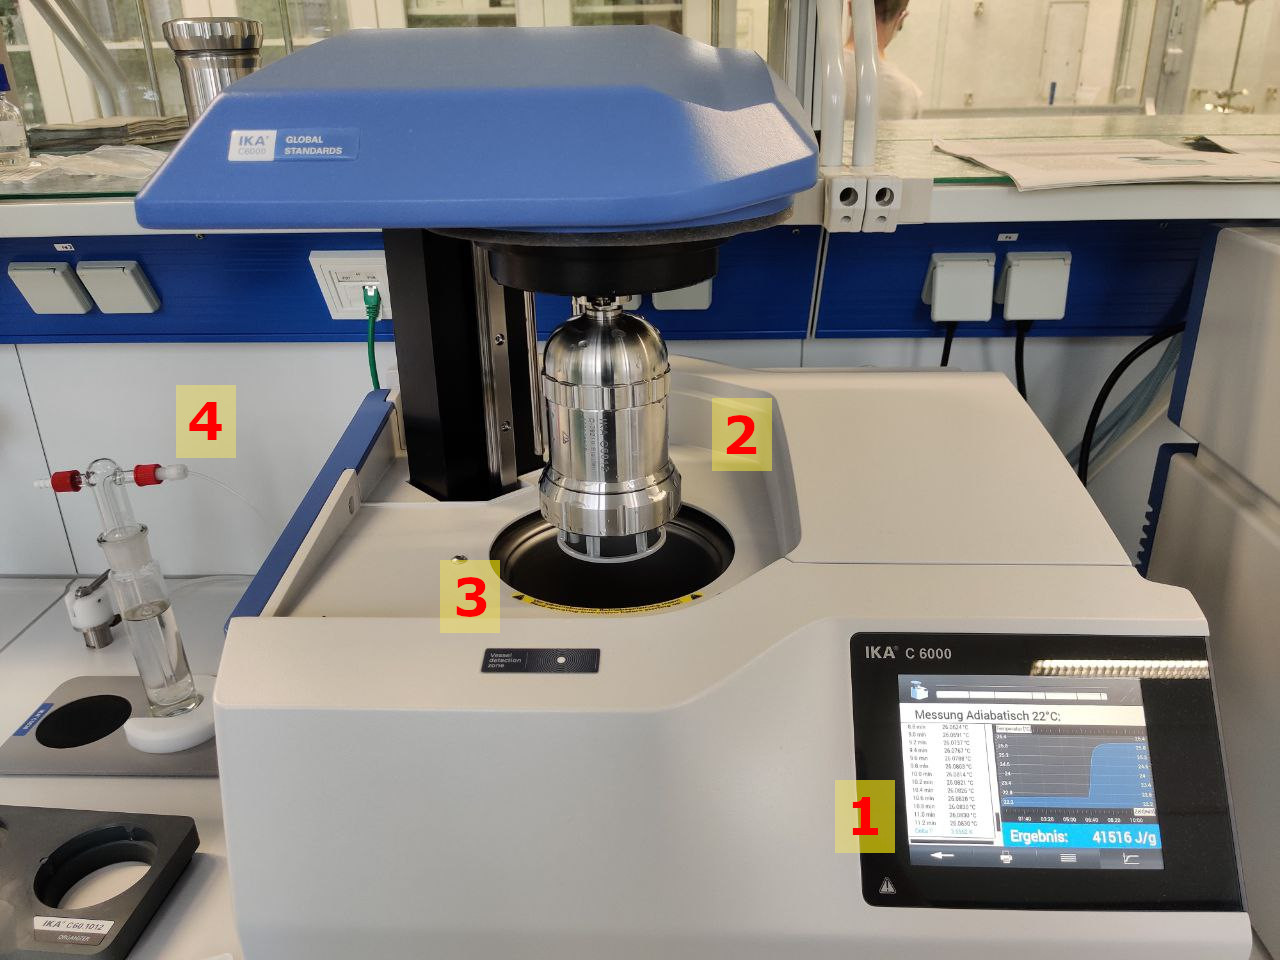
\includegraphics[width=.7\textwidth]{assets/photos/kaloriemeter_aufbau_edit.jpg}
			\caption[Im Versuch verwendetes Kalorimeter]{Im Versuch verwendetes Kalorimeter C 6000 der Firma \textsc{IKA}. Zu sehen 1: Bedienfeld, 2: Druckbehälter, 3: Innenkessel, 4: Entlüftungsstation.}
			\label{fig:kalorimeter aufbau}
		\end{figure}
		Das Funktionsprinzip besteht hierbei aus einer sehr genauen Messung der Temperaturerhöhung eines die Verbrennungskammer umfließenden
		Wassers. Da es hierbei unweigerlich auch Wärmemengenverlusten an den Gefäßwenden, Leitungen und dergleichen kommt, muss,
		um entsprechende Kompensationen durchführen zu können, im Vorfeld jeder Messung eine Kalibrierung durchgeführt werden.
		Die Kalibrierung bestimmt hier die Wärmekapazität der Messeinrichtung selbst und folgt der kalorischen Grundgleichung \cref{eq:kalorische grundgleichung} \cite{Einstieg.in.die.Physikalische.Chemie.fuer.Nebenfaechler.Bechmann.2016}.
		\begin{equation}
			Q = \Delta T \cdot k = \Delta T \cdot \sum_i c_i \cdot m_i
			\label{eq:kalorische grundgleichung}
		\end{equation}

		\(k = \sum_i c_i \cdot m_i\) bezeichnet hier einen systemspezifischen Proportionalitätsfaktor, der die kumulierte Fähigkeit der einzelnen Systemkomponenenten Wärme aufzunehmen
		widerspiegelt und muss durch Kalibrierung ermittelt werden. \(Q\) ist hier die zugeführte Wärmemenge und \(\Delta T\) die zu messende Temperaturänderung.\par\medskip
		\begin{figure}[h]
			\centering
			\includesvg[width=.6\textwidth]{assets/svg/paraffin_rein_struktur}
			\caption[Exemplarische Strukturformel reinen Paraffins]{Exemplarische Strukturformel reinen Paraffins.}
			\label{fig:paraffin rein}
		\end{figure}
		Sowohl die eigentliche Messung als auch die Kalibrierung finden unter Zufuhr reinen Sauerstoffs statt. Hierbei wird, wie eingangs bereits erwähnt, das Präparat
		vollständig verbrannt während die Temperaturänderung des umliegenden Wassers konstant gemessen wird.
		\Cref{fig:paraffin rein} und \ref{fig:paraffin ckw} zeigen exemplarische Strukturformeln jeweils eines reinen und eines mit Chlor modifizierten
		Paraffins.
		\begin{figure}[h]
			\centering
			\includesvg[width=.6\textwidth]{assets/svg/paraffin_ckw_struktur}
			\caption[Exemplarische Strukturformel eines mit Chlor verunreinigten Paraffins]{Exemplarische Strukturformel eines mit Chlor verunreinigten Paraffins.}
			\label{fig:paraffin ckw}
		\end{figure}\\
		Das in der kalorimetrischen Bestimmung verwendete Präparat ist ein Paraffin zweiten Typs. So wird beim Versuch über die Bestimmung des Brennwertes des
		Präparates hinaus auch der angelagerte Chlorgehalt bestimmt. Dies geschieht in einer nachgelagerten konduktometrischen Fällungstitration, die in \cref{sec:titration}
		näher erläutert werden soll.\par\medskip
		Um den beim Aufschluss zu erwartenden Chlorwasserstoff aufzufangen wird in Vorbereitung \SI{100}{mL} 0,1 molarer Natronlauge hergestellt.
		\begin{equation}
			\frac{c_{soll}(NaOH)}{V_{soll}} = \frac{c_1(NaOH)}{V} \qquad \Leftrightarrow \qquad V = c_1(NaOH) \cdot \frac{V_{soll}}{c_{soll}(NaOH)}
			\label{eq:verduennung}
		\end{equation}\\
		Im Versuch steht 1 molare Natronlauge zur Verfügung aus der die gewünschte Konzentration \(c_{soll}(NaOH)\) durch Verdünnung hergestellt werden muss. \Cref{eq:verduennung}
		folgend errechnet sich die zu entnehmende Menge zu \(V = \SI{10}{mL}\). Mit einer Vollpipette vorsichtig entnommen und in einen Messkolben überführt wird die Differenz
		zum Sollvolumen mit \SI{90}{mL} VE-Wasser aufgefüllt.\par\medskip
		%
		Die oben beschriebene Kalibrierung wird im Versuch durch Verbrennung von \SI{0,5}{g} Benzoesäure durchgeführt wobei die Kalibrierparameter

		\begin{addmargin}[8mm]{0pt}
			\texttt{Bezugsbrennwert}\\
			\texttt{Einwaage} und\\
			\texttt{QFremd1/2}
		\end{addmargin}
		bekannt sein müssen. \texttt{Bezugsbrennwert} ergibt sich aus dem spezifischen Brennwert der Benzoesäure mit \(H_0 = \SI{26,455}{\kilo\joule\per\kelvin}\) \cite{Versuchsanleitung.phys.chemie}.
		Die in Tablettenform vorgelegten Benzoesäure wird auf der Laborwaage im Tiegel eingewogen und ergibt so den Parameter \texttt{Einwaage} mit \(m_{Benz} = \SI{(506,8 \pm 1)}{mg}\).
		Ein sich ebenfalls im Tiegel befindlicher Baumwollfaden wird elektrisch entzündet und startet so die Verbrennung. Hierdurch werden allerdings zwei weitere Wärmeenergien eingebracht
		die durch Angabe des letzten Parameters \texttt{QFremd1/2} intern kompensiert werden. Hier wird \SI{120}{J} (Summe aus der Verbrennungsenergie des Baumwollfadens mit \(Q_{faden} = \SI{50}{J}\) und der
		des Zündfunkens mit \(Q_{funke} = \SI{70}{J})\) hinterlegt. Letztlich kann für die Kalibrierung ausgehend von \cref{eq:kalorische grundgleichung} geschrieben werden:
		\begin{equation}
			Q = H_0 \cdot m_{Benz} + Q_{faden} + Q_{funke} = \Delta T \cdot k
			\label{eq:grundgleichung fuer kalib umgeschrieben}
		\end{equation}

		mit \(k\) als der einzigen Unbekannten.\par
		Die im Zuge der Vorbereitung gemessene Kalorimeterkonstante \(k\) ergab sich zu
		\begin{equation}
			k = \SI{8025}{\joule\per\kelvin}
			\label{eq:kalorimeterkonstante}
		\end{equation}

		womit bei nachfolgenden Messungen der spezifische Brennwert \(H_0\) der unbekannten Probe ermittelt werden kann.
	\section{Konduktometrische Titration}\label{sec:titration}
		Liegt in einer Lösung nur eine Ionenart vor, so kann durch Neutralisation mit begleitender Überwachung der Leitfähigkeit der Lösung
		auf die anfängliche Ionenkonzentration geschlossen werden.

		Die Leitfähigkeit einer Lösung hängt in erster Linie von der Ionenbeweglichkeit (die wiederum in gewissem Maße auch von der Temperatur abhängt) und
		-konzentration ab. Die Leitfähigkeit hat dort ein Minimum, wo bei der Neutralisation ein Äquivalenzpunkt erreicht wird.
		Im vorliegenden Versuch wird nach dieser Methode der Chloridgehalt des Residuums aus Versuch 11 mittels Neutralisation mit einer Silbernitratlösung bestimmt.
		Da hierzu die Ionenkonzentration des Titranten möglichst genau bekannt sein muss, wird vorbereitend eine Lösung bekannten Chloridgehalts
		titriert. \nocite{Analytische.Chemie.I.Ritgen.2019}
		\begin{reaction}
			Na_{(aq)}^{+}Cl_{(aq)}^{-} + Ag_{(aq)}^{+}NO_{3(aq)}^{-} -> AgCl v + Na_{(aq)}^{+} + NO_{3(aq)}^{-} "\label{re:NaCl und AgNO3}"
		\end{reaction}
		\subsection{Lösung bekannten Chloridgehaltes}\label{sec:bekannter chloridgehalt}
			Zur Herstellung einer Lösung bekannten Chloridgehalts wird Natriumchlorid (Kochsalz) auf der Laborwaage möglichst genau eingewogen
			und in einem Messkolben durch Auffüllen mit VE-Wasser gelöst. Ziel ist eine Chloridkonzentration von \(c(Cl^{-}) \approx \SI{0,1}{\mole\per\litre}\).
			\begin{equation}
				m = \left[M(Cl^{-}) + M(Na^{+})\right] \cdot c(Cl^{-}) \cdot V
				\label{eq:masse NaCl}
			\end{equation}

			Mit den molaren Massen von \(M(Cl^{-}) \approx \SI{35,450}{\gram\per\mole}\) und \(M(Na^{+}) \approx \SI{22,98977}{\gram\per\mole}\) sowie
			dem herzustellenden Volumen von \(V = \SI{50}{\milli\litre}\) ergibt sich mit \cref{eq:masse NaCl} eine einzuwiegende Masse des Salzes
			von gemäß \SI{292,2}{mg}. Mit einer tatsächlich eingewogenen Masse von\\
			\(\SI{(298,8 \pm 0,1)}{\milli\gram}\) führt dies wiederum gemäß \cref{eq:konzentration Cl}
			\begin{equation}
				c(Cl^-) = \frac{M(Cl^-)}{M(Cl^-) + M(Na^+)} \cdot \frac{m}{M(Cl^-) \cdot V}
				\label{eq:konzentration Cl}
			\end{equation}
			zu einer Konzentration von \(c(Cl^{-}) \approx \SI{0,1023}{\mole\per\litre}\).\par
			Von der hergestellten Lösung werden \SI{25}{\milli\litre} entnommen und innerhalb eines Becherglases mit \SI{200}{\milli\litre}
			VE-Wasser verdünnt.
		\subsection{Titerbestimmung}\label{sec:titerbestimmung}
			Das Becherglas aus \cref{sec:bekannter chloridgehalt} wird mit einem Rührstäbchen versehen auf einen Magnetrührer gestellt und
			das in einem Stab kombinierte Elektrodenpaar des Konduktometers in einem über dem Becherglas befindlichen Stativ so arretiert, dass
			die Kontaktflächen der Elektroden möglichst tief in die Lösung eintauchen\footnote{Hierbei ist darauf zu achten, dass der Elektrodenstab möglichst frei von Kontamination ist.}.

			Nach Einschalten des Magnetrührers wird \SI{2}{\milli\litre}-Schritten Silbernitratlösung zu titriert und bei jedem Titrationsschritt die
			momentane Leitfähigkeit der Lösung am Konduktometer abgelesen und aufgezeichnet. Nahe des Äquivalenzpunktes werden die Titrationsschritte auf
			etwa \SI{0,5}{\milli\litre} reduziert um das Minimum der Leitfähigkeit möglichst genau zu lokalisieren. Ist der Äquivalenzpunkt erreicht wird die Schrittweite
			der Titration wieder erhöht und so lange Silbernitratlösung zugegeben, bis etwa \SI{20}{\milli\litre} nach dem Äquivalenzpunkt verbraucht sind.
%ltex: language=de-DE
\chapter{Fazit}
	Der Praktikumsversuch hat gezeigt, dass sich zumindest beim untersuchte Spannungsinverter die Wahl der passiven Beschaltung
	drastisch auf die Performance der Schaltung auswirken kann.\par\medskip
	Beim Versuch selbst war die größte Hürde das Simulationsprogramm selbst. So wurden Simulationen bisweilen nie abgeschlossen,
	Wellenformen wurde bei wiederholter Simulation aber ohne Veränderung der Parameter verschieden ausgegeben und ein mal
	kam es sogar zu einem Absturz des Programms. Dies ist in der Form bisher noch nicht passiert. Eine kurze Recherche deutet darauf hin,
	dass eine ungünstige Parametrisierung der Komponenten der Bibliothek und/oder der untersuchten Schaltung in manchen Fällen
	zu unvorhergesehenem Verhalten führen kann \cite{ltspice.bug}.\par
	Als Workaround wurde sämtlichen Simulationsanweisungen \texttt{uic} hinzugefügt, was das Problem zumindest augenscheinlich lösen konnte.\par\medskip
	Auch die Anleitung zum Praktikumsversuch war diesmal weniger gut verständlich. So wurde etwa \(\Delta U_{aus}\) nicht konsequent
	für den gleichen Sachverhalt verwendet oder es war bisweilen nicht sofort ersichtlich, was konkret gemessen werden soll.\par\medskip
	Zuletzt ist zu sagen, dass hier zwar die Verwendbarkeit in etwa eigenen Projekten noch fraglich ist, es aber nicht schaden kann das Bauteil
	und seine Charakteristika im Hinterkopf zu behalten.
%ltex: language=de-DE
\chapter{Auswertung}
	Hier soll zunächst aus den gesammelten Messdaten der spezifische Brennwert \(H_0\) der unbekannten Probe ermittelt werden. Im darauf folgenden
	Kapitel wird der in der Probe gebundene Chlorgehalt ermittelt.
	\section{Kalorimetrie}
		Die Messergebnisse aus der in \cref{sec:vorbereitung kalorimetrischer aufschluss} durchgeführten Kalibrierung und der in
		\cref{sec:kalorimeter bestimmung unbekannte probe} beschriebenen Folgemessung des Paraffins sind in \cref{fig:tempverlauf}
		grafisch aufgetragen.
		\begin{figure}[h]
			\centering
			\includesvg[width=.9\textwidth]{assets/plots/kalo/kalo}
			\caption[Temperaturverlauf der Kalibrierung und der Messung]{Temperaturverlauf beim Kalibriervorgang (blau) und bei der Messung der probe (rot).}
			\label{fig:tempverlauf}
		\end{figure}

		Mit der nach \cref{eq:kalorimeterkonstante} ermittelten Kalorimeterkonstante wird durch Umstellen von \cref{eq:grundgleichung fuer kalib umgeschrieben}
		der Brennwert der Probe ermittelt gemäß
		\begin{equation}
			H_0 = \frac{\Delta T \cdot k - Q_{faden} - Q_{funke}}{m_{tot}}
			\label{eq:brennwertgleichung}
		\end{equation}
		und errechnet sich mit \(\Delta T = \SI{3,5619}{\kelvin}\), \(m_{tot} = \SI{688,8}{\milli\gram}\) und dem in \cref{eq:kalorimeterkonstante} gefundenen Wert für \(k\)
		zu
		\begin{align}
			H_0	&= \frac{\SI{3,5619}{\kelvin} \cdot \SI{8,025}{\kilo\joule\per\kelvin} - \SI{0,050}{\kilo\joule} - \SI{0,070}{\kilo\joule}}{\SI{688,8 \cdot 10^{-6}}{\kilo\gram}}\nonumber\\
				&= \SI{41,3244}{\mega\joule\per\kilo\gram}
		\end{align}
	\section{Titration}
		Mit dem Verbrauch des Titers in der in \cref{sec:bekannter chloridgehalt} hergestellten Lösung bis zum Äquivalenzpunkt
		lässt sich die Konzentration der Silber-Anionen \(c(Ag^{+})\) des Titers bestimmen. \Cref{fig:verlauf leitf chloridlsgn}
		zeigt die aufgezeichneten Datenpunkte und die beiden Ausgleichsgeraden. Das Verbrauchsvolumen in ihrem Schnittpunkt beträgt hier etwa
		\SI{24,788}{\milli\litre}.
		\begin{figure}[h]
			\centering
			\includesvg[width=.9\textwidth]{assets/plots/titration/chloridlsgn}
			\caption[Verlauf der Leitfähigkeit verdünnter Benzoesäure]{Verlauf der Leitfähigkeit bei der konduktometrischen Titration der Referenzlösung.}
			\label{fig:verlauf leitf chloridlsgn}
		\end{figure}

		Zunächst muss die Anzahl vorgelegter Chlorid-Ionen bekannt sein:
		\begin{align}
			n(Cl^-) &= c(Cl^-) \cdot V_{Titrant,1}\nonumber\\
					&= \SI{0,1}{\mole\per\litre} \cdot \SI{25}{\milli\litre} = \SI{2,5}{\milli\mole}\label{eq:anzahl chloridionen}
		\end{align}
		Mit \(n(Cl^{-}) = n(Ag^{+})\) (vgl. \cref{eq:grundgleichung fuer kalib umgeschrieben}) ergibt sich die Konzentration der
		Silbernitratlösung rechnerisch zu
		\begin{align}
			c(Ag^+)	&= \frac{n(Ag^+)}{V_{Titer,1}} = \frac{n(Cl^-)}{V_{Titer,1}}\nonumber\\
					&= \frac{\SI{2,5}{\milli\mole}}{\SI{24,788}{\milli\litre}}\nonumber\\
					&\approx \SI{0,10}{\mole\per\litre}
			\label{eq:konzentration silber gerechnet}
		\end{align}

		Somit lässt sich nach Titration der chlorierten Absorberlösung (vgl. \cref{fig:verlauf leitf aufschluss}) mit Umstellen von \cref{eq:konzentration silber gerechnet}
		die Anzahl der in Lösung befindlichen Chlorid-Ionen
		\begin{align}
			\setlength{\jot}{10pt}
			n(Cl^-)	&= c(Cl^-) \cdot V_{Titer,2}\nonumber\\
					&= \SI{0,1}{\mole\per\litre} \cdot \SI{9,461}{\milli\litre}\nonumber\\
					&\approx \SI{0,95}{\milli\mole}
			\label{eq:anzahl chlor in absorber}
		\end{align}
		und weiterführend mit der Einwaage von \(m_{tot} = \SI{688,8}{\milli\gram}\) des verbrannten Paraffins sein Chlorgehalt bestimmen.
		\begin{align}
			p(Cl^-) &= \frac{m_{Cl^-}}{m_{tot}} \cdot \SI{100}{\percent} = \frac{M(Cl^-) \cdot n(Cl^-)}{m_{tot}} \cdot \SI{100}{\percent}\nonumber\\
					&= \frac{\SI{35,45}{\gram\per\mole} \cdot \SI{0,95}{\milli\mole}}{\SI{688,8}{\milli\gram}} \cdot \SI{100}{\percent}\nonumber\\
					&\approx \SI{4,9}{\percent}
		\end{align}
		\begin{figure}[h]
			\centering
			\includesvg[width=.9\textwidth]{assets/plots/titration/absorb}
			\caption[Verlauf der Leitfähigkeit des Aufschlusses]{Verlauf der Leitfähigkeit bei der konduktometrischen Titration des in NaOH gebundenen Aufschlusses aus V11.}
			\label{fig:verlauf leitf aufschluss}
		\end{figure}
\chapter{5}
%-----------------------------------------------------------------
\newpage
\listoffigures 
% \listoftables
\addchap{Glossar}
\begin{table}[h]
    \begin{tabular}{@{}ll@{}}%
        \(C\) & Kapazität \SI{}{\farad}\\
        \(I_{load}\) & Laststrom \SI{}{A}\\
        \(P\) & Leistung \SI{}{W}\\
        \(R_i\) & Innenwiderstand \SI{}{\ohm}\\
        \(T\) & Periodendauer \SI{}{\second}\\
        \(U_{in}\) & Eingangsspannung \SI{}{V}\\
        \(U_{loss}\) & Spannungsverlust im ungeregelten Fall \SI{}{V}\\
        \(U_{out}\) & Ausgangsspannung des Netzteils \SI{}{V}\\
        & \\
        \(f\) & Frequenz \SI{}{\hertz}\\
        & \\
        \(\eta\) & Wirkungsgrad\\
    \end{tabular}
    \label{tab:glossar}
\end{table}
\appendix
% %LTeX: language=DE
\chapter{Externe Referenzen}
	
\chapter{Anhang}
	\begin{lstlisting}[style=python, caption={Zur Auswertung der konduktometrischen Titration verwendeter Python-Code.}]
		import matplotlib.pyplot as plt
		import numpy as np
		import pandas as pd
		from scipy.optimize import curve_fit
		import os

		sample_files = os.listdir("messdaten/csv_titration/")
		print(sample_files)

		spl_lst = []
		for i,file in enumerate(sample_files):
			with open(("messdaten/csv_titration/" + file), newline='', encoding='utf-8') as path:
				frame = pd.read_csv(path, delimiter=';')
				frame.columns = [col.strip() for col in frame] # stupid whitespaces t(-_-t)
				spl_lst.append(frame)
				del frame

		absorb = spl_lst[0]
		known = spl_lst[1]
		absorb_vol = np.array(absorb["Vol. Maßlösung / [mL]"])
		absorb_leit = np.array(absorb["Leitfähigkeit / [mS/cm]"])
		known_vol = np.array(known["Vol. Maßlösung / [mL]"])
		known_leit = np.array(known["Leitfähigkeit / [uS/cm]"])

		def func(x, m, b):
			return x*m+b

		def findx(m, b, n, c):
			return (b - c)/(n - m)

		cm = 1/2.54 # inch to cm, metric like brrr

		plt.style.use("default")
		plt.style.use("seaborn-paper")

		fig1, ax1 = plt.subplots(figsize=(20*cm, 20*(9/16)*cm))

		ax1.scatter(absorb["Vol. Maßlösung / [mL]"], absorb["Leitfähigkeit / [mS/cm]"],
		marker="x", linewidth=.6, label="Datenpunkte")
		popt, pcov = curve_fit(func, np.array(absorb_vol[0:np.argmin(absorb_leit)-1]), np.array(absorb_leit[0:np.argmin(absorb_leit)-1]))
		m, b = popt
		ax1.plot(np.array(absorb_vol[0:np.argmin(absorb_leit)+8]),
		func(np.array(absorb_vol[0:np.argmin(absorb_leit)+8]), *popt),
		color="#800000", linestyle="--", label="Lin. Fit")
		popt, pcov = curve_fit(func, np.array(absorb_vol[np.argmin(absorb_leit)-1:]), np.array(absorb_leit[np.argmin(absorb_leit)-1:]))
		n, c = popt
		ax1.plot(np.array(absorb_vol[np.argmin(absorb_leit)-2:]),
		func(np.array(absorb_vol[np.argmin(absorb_leit)-2:]) ,*popt),
		color="#800000", linestyle="--")
		ax1.axvline(findx(m, b, n, c), lw=0.5, color="#800000", label="Verbr. Vol. $\\approx$ 9.461 mL")

		ax1.set_title("Verlauf der Leitfähigkeit - Absorberlösung aus V11", fontsize=12)
		ax1.set_xticks(np.arange(0,23,2))
		ax1.set_xlabel("Vol. Maßlösung / $mL$", fontsize=8)
		ax1.set_ylabel("Leitfähigkeit / $\\frac{mS}{cm}$", fontsize=8)
		ax1.legend()
		ax1.grid(axis='both', alpha=.3)
		#========================================================
		fig2, ax2 = plt.subplots(figsize=(20*cm, 20*(9/16)*cm))

		ax2.scatter(known["Vol. Maßlösung / [mL]"], known["Leitfähigkeit / [uS/cm]"],
		marker="x", linewidth=.6, label="Datenpunkte")
		popt, pcov = curve_fit(func, np.array(known_vol[0:np.argmin(known_leit)-1]), np.array(known_leit[0:np.argmin(known_leit)-1]))
		m, b = popt
		ax2.plot(np.array(known_vol[0:np.argmin(known_leit)+4]),
		func(np.array(known_vol[0:np.argmin(known_leit)+4]), *popt),
		color="#800000", linestyle="--", label="Lin. Fit")
		popt, pcov = curve_fit(func, np.array(known_vol[np.argmin(known_leit):]), np.array(known_leit[np.argmin(known_leit):]))
		n, c = popt
		ax2.plot(np.array(known_vol[np.argmin(known_leit)-1:]),
		func(np.array(known_vol[np.argmin(known_leit)-1:]) ,*popt),
		color="#800000", linestyle="--")
		ax2.axvline(findx(m, b, n, c), lw=0.5, color="#800000", label="Verbr. Vol. $\\approx$ 24.788 mL")
		# print(findx(m, b, n, c))

		ax2.set_title("Verlauf der Leitfähigkeit - Chloridlösung", fontsize=12)
		ax2.set_xticks(np.arange(0,46,5))
		ax2.set_xlabel("Vol. Maßlösung / $mL$", fontsize=8)
		ax2.set_ylabel("Leitfähigkeit / $\\frac{\\mu S}{cm}$", fontsize=8)
		ax2.legend()
		ax2.grid(axis='both', alpha=.3)

		plt.tight_layout()
		plt.show()
	\end{lstlisting}
	\clearpage
	\begin{lstlisting}[style=python, caption={Zur Auswertung der kalorimetrischen Messung verwendeter Python-Code.}]
		import matplotlib.pyplot as plt
		import numpy as np
		import pandas as pd
		from scipy.optimize import curve_fit
		import os

		sample_files = os.listdir("messdaten/csv_kalo/")
		print(sample_files)

		spl_lst = []
		for i,file in enumerate(sample_files):
			with open(("messdaten/csv_kalo/" + file), newline='', encoding='utf-8') as path:
				frame = pd.read_csv(path, delimiter=';')
				frame.columns = [col.strip() for col in frame] # whitespaces, again! double t(-_-t)
				spl_lst.append(frame)
				del frame

		kalib = spl_lst[0]
		benzo = spl_lst[1]
		kalib_zeit = np.array(kalib["Zeit"] * 60)
		kalib_temp = np.array(kalib["Temp"] + 273.15)
		benzo_zeit = np.array(benzo["Zeit"] * 60)
		benzo_temp = np.array(benzo["Temp"] + 273.15)
		
		cm = 1/2.54 # inch to cm, metric like brrr

		plt.style.use("seaborn-paper")

		fig1, ax1 = plt.subplots(figsize=(20*cm, 20*(9/16)*cm))

		ax1.plot(kalib_zeit, kalib_temp,
		label=("Kalibrierung, $\Delta T = {:.4f}K$".format(np.max(kalib_temp)-np.min(kalib_temp))))
		ax1.plot(benzo_zeit, benzo_temp,
		label=("Probe, $\Delta T = {:.4f}K$".format(np.max(benzo_temp)-np.min(benzo_temp))), color="#800000")

		ax1.set_title("Temperaturänderung der kalorimetrischen Bestimmung", fontsize=12)
		ax1.set_xlabel("Zeit / [s]", fontsize=8)
		ax1.set_ylabel("Temperatur / [K]", fontsize=8)
		ax1.axhline(np.min(kalib_temp), linestyle="--", lw=.5)
		ax1.axhline(np.max(kalib_temp), linestyle="--", lw=.5)
		ax1.axhline(np.min(benzo_temp), linestyle="--", lw=.5, color="#800000")
		ax1.axhline(np.max(benzo_temp), linestyle="--", lw=.5, color="#800000")
		ax1.legend(loc=4)
		ax1.grid(axis='both', alpha=.3)

		plt.tight_layout()
		plt.show()
	\end{lstlisting}
\printbibliography
%=================================================================
\end{document}